\documentclass[11pt]{article}
\usepackage{graphicx, float}
\parindent=0in
\parskip=8pt
\begin{document}
\title{COMP 512 - Final Project Report}
\author{Luke Emery-Fertitta - Student ID: 260569374 \\ Jonathan Campbell - Student ID: 260481285}
\date{2015 December 3}
\maketitle

\section*{General design & architecture}

To distribute load over several servers, we created a middleware to communicate between the client and resource manager (RM) servers. The middleware will receive requests from the client and forward them to the appropriate resource manager server, each server being responsible for one resource. The middleware is also responsible for customer data, since it is assumed that the most popular transactions performed will include modification or reading of customer data.  \par

\section*{Performance results}

\subsection*{Technique}

For both parts, we use testing clients that repeatedly submit two transaction types. One is a middle-ware only transaction containing three customer read operations and three write operations. The other uses all three resource managers, performing a read and a write at each one. Each experiment can have the number of clients and delay between transactions varied, allowing us to control transactions per second.

\subsection*{Results}

\begin{table}[H]
\centering
\caption{Performance of Single-Client Txn}
\begin{tabular}{c|c}
Type & Average Response Time(s) \\
\hline
Local MW & 0.0445 \\
Local RM & 0.1000 \\
Network MW & 0.0915 \\
Network RM & 0.1704 \\
\end{tabular}
\end{table}

\begin{figure}[H]
\centering
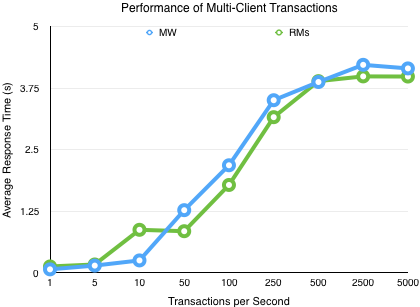
\includegraphics[scale=1]{plot.png}
\end{figure}

\subsection*{Analysis}

\textbf{Single-Client Observations:} \\
Network operations take roughly twice as long as local operations. RM transactions take roughly twice as long as their MW counterparts.\par

\textbf{Single-Client Analysis:} \\
There is network latency, and increased message hops for RM transactions. \par

\textbf{Multi-Client Observation:}\\
Initially, RM-only transactions have a longer average response time than MW-only transactions. This swaps near 40 tps. After that, both increase at steady exponential rate (due to the logarithmic $x$-axis scale) with MW-only transactions being a constant amount above RM. At 500 transactions per second these amounts converge, followed by a slight increase in the response time on the part of the middleware. Both converge and plateau at 5000 transactions per second. \par

\textbf{Multi-Client Analysis:}\\
Between 1 and 40 tps, the RM transactions take longer due to the message transfer overhead. This may be a bit extreme at 10 tps and could be slightly exaggerated by noise. After this, the limiting factor is the bottlenecking due to lock conflicts, which continues to become more severe. There may also be network congestion, contributing to the increase to a lesser degree. Finally, the plateau occurs due to the limitation on the Java client. We can only send so many transactions per second, so although we set the parameters for 10,000 tps, we are unable to actually achieve that number. Due to this insufficiency, we are capped in the number of transactions per second that can be tested.

\section*{Data design}

\section*{Implementation of features}

\subsection*{Middleware}

The middleware system uses a new class that implements ResourceManager, and which maintains one WSClient for each resource manager server (flight, car, and room) for communication. Requests from the client are received through the Web Services interface. Each ResourceManager method involving flight, car, or room data will communicate with the appropriate Resource Manager using the relevant WSClient to invoke the smae method on that server.  \par

The middleware also maintains by itself all customer-related data in a hashtable. Methods that involve only customer data are processed directly at the middleware layer without any connection to an RM. Methods that involve both customer data and flight/car/room data, such as the reservation methods, or deleteCustomer, involve both processing by the middleware layer and communication with the appropriate resource managers.  \par

Since the middleware and server use the same class interface, the client can acquire the WSDL file from either. We chose to get it from the middleware so that the client doesn't need to know any information about the RM servers themselves.  \par

The middleware receives information about the RM servers (port and hostname) on server startup, through environment variables in the web.xml file.  \par


\section*{Special features}

\section*{Concurrency control}

\section*{Problems encountered}

One problem that was encountered that originated from the centralized model was the management of undo functions. Since the middleware contains the transaction manager, it is also responsible for informing the TM of the undo operations to perform in case of abort, before the actual operation takes place. Therefore, the middleware will need to know the reverse of each operation, even when it is only forwarding the operation to a resource manager. The undo operations are hardcoded in the middleware, so knowledge about each operation must reside at both middleware and RMs, which breaks the pattern of functional isolation. Further, some undo operations are more complex, in cases where an operation (like addFlight) can have different effects based on data state (it can add a completely new flight, or edit details of a current flight), leading to a necessity for state analysis on the middleware and communication with the RM to determine which action will be performed, in order to record the correct undo operation. \par

Concurrency was a concern due to the multithreaded request handling and asynchronus requirements of the transaction manager. We had to ensure that the transaction identifier was unique regardless of \texttt{start} execution order, and that once a shutdown request has been initiated, no client is able to start a new transaction. The former problem was solved with an \texttt{AtomicInteger} attribute, which allows for an atomic get and increment. The latter problem was solved by synchronizing the shutdown and start methods and adding an \texttt{isShutdown} attribute, such that once the shutdown has begun, threads will block at \texttt{start}, and after it finishes, transactions will fail to start. \par

\section*{Testing}

\subsection*{Middleware}

Testing of the middleware was initially done manually, followed by a short series of JUnit tests. These tests act as an automated client, running a list of commands and verifying the results with assertions. This allows us to run detailed tests frequently, and without having to rely on human verification.  \par

\subsection*{Lock Manager}

To test the lock manager, we created a framework to easily specify transactions and their specific operations to be executed. A Transaction Simulation class (TxnSimul) receives as input a series of integers representing the operations that the transaction should execute, with each group of four integers specifying the transaction ID, data item, lock type (read or write), and the amount of seconds to sleep after executing the operation. With this latter argument, it is possible to interleave the operations of two different transactions. The TxnSimul objects once created are inserted into an array, and then a new thread is created for each, so that all run concurrently. We created several tests in this format to verify the integrity of the lock manager, including the following schedules, with reasoning for each:

\begin{itemize}
\item T1 reads A, T1 writes A, T1 commit (lock conversion)
\item T1 reads A, T2 reads B, T2 writes A, T1 writes B, T1 commit, T2 commit (deadlock detection)
\item T1 reads A, T2 reads A, T2 commit, T1 writes A, T1 commit (check that read lock can be acquired on object with read lock already, and unlocking of locks upon commit)
\item T1 reads A, T2 reads A, T1 writes A, T1 commit, T2 commit (check if shared lock blocks other's write)
\end{itemize}

Specific particularities of scheduling prevented by two-phase locking such as dirty reads, writes, unrepeatable reads, etc., were not tested here since it was assumed that the provided 2PL locking implementation was sound. \par

\subsection*{Transaction Manager}

With regards to testing of the transaction manager, sequences of commands were manually inputted into the client console with verification of results. Testing of undo operations was of particular focus, as well as concurrent modification situations (to verify correctness of locks).\par


\end{document}
